% !TeX encoding = UTF-8
% !TeX program = pdflatex

\documentclass[11pt]{article}
\usepackage{graphicx}

\newcommand\CIPH{C\!I\!P\!H_K}

\title{{\bf Comparison of Symmetric Ciphers in OpenSSL} \\ \bigskip \large HW1 - CNS Sapienza}
\date{2019-11-4}
\author{Valerio Coretti 1635747}
\pagenumbering{roman}

\begin{document}
\maketitle

\section{Introduction}
Data encryption procedures are divided into two categories: {\em Symmetric encryption} and {\em Asymmetric encryption}. These techniques depending on the type of security keys used to encrypt/decrypt. In this paper, we focused on Symmetric Encryption. In this type of encryption, 
the sender and the receiver first agree on a secret {\em "shared"} key, then they use this secret key to encrypt and decrypt their messages.

{\em Block Ciphers} are widely used in symmetric encryption. A block cipher consists of an encryption algorithm and a decryption algorithm. 
These algorithms take a fixed-length messages, called {\em blocks}, a variable-length {\em key}, and through {\em Operating Modes}, generate
a ciphertext. Modes of operations are the techniques used to encrypt messages larger than a single block.

In the following sections, we will present a fair comparison between four of the most common Block Ciphers: 
{\em RC2}, {\em DES}, {\em Blowfish} and {\em AES}, based on three different operating modes: {\em CBC}, {\em ECB} and {\em OFB}.
In particular, we will trie to answer to this question: given a pair (cipher, operating mode) is encryption faster or slower than decryption?

\section{Preliminary Choices}
To answer the above question we have chosen to measure the encryption/decryption speeds on files of different sizes: 1MB, 10MB, 100MB, 300MB.
The main parameter on which we based our analysis is the {\em Average Speed Ratio}.

$ Average Speed Ratio = (AvgSpeedEncyption)/(AvgSpeedDecryption) $

The average is calculated on five encryption and five decryption of the same file.

Moreover, the following table shows the settings of the algorithm used in this experiment.

\bigskip
\begin{tabular}{ | l | l | l | }
        \hline
        \textbf{Cipher} & \textbf{Key Size (Bits)} & \textbf{Block Size (Bits)} \\ \hline
    AES & 128 & 128  \\ \hline
    DES & 64 & 64 \\ \hline
    Blowfish & 128 & 64 \\ \hline
    RC2 & 128 & 64 \\ \hline
\end{tabular}
\bigskip

The comparison has been conducted with the OpenSSL library using C language with Linux Mint and over an Intel core i5 64bit processor with 4GB of RAM.

\subsection{OpenSSL: Standard Function vs EVP interface}
\begin{quote}
OpenSSL is a software library for applications that secure communications over computer networks against eavesdropping or need to identify the party at the other end. {\em Wikipedia}
\end{quote}
This library has two main sets of function to perform the various cipher algorithms with the related operating modes: 
{\em Standard Function} and {\em EVP interface}. Standard Function is the first set of instructions released by OpenSSL and, as we will see, these are slow and not optimized, especially with cipher AES and CBC mode. Instead, the EVP functions provide a high-level interface to cryptographic functions. 

In this paper first, we will discuss the results with the standard functions and then we will see the improvements obtained with EVP.

\section{Evaluation Methodology}
We have used two Simulations Programs, one for Standard Function and one for EVP. Both take one input parameter that is the file to encrypt and returns all the times-speed for every cipher and related operating modes. Key and IV used are pseudo-randomly generated. Example of output (only for AES):

\begin{figure}[!ht]
  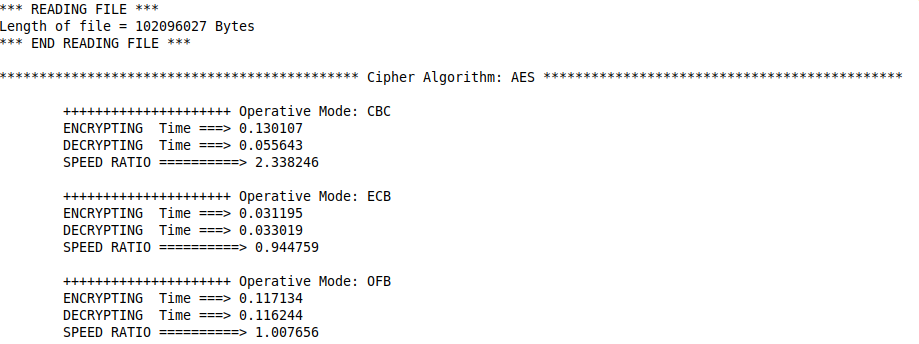
\includegraphics[width=1\textwidth]{pic1-hw1-1635747}
  \label{fig:Example of output with EVP}
\end{figure}

\newpage
\section{Simulation Results}
This section will discuss graphics results obtained from running the simulation program for Standard functions and EVP. We will show graphics three different graphics, one for every operating mode.

\subsection{Standard functions results}
We begin our analysis with CBC. From the graph, we immediately notice a surprising thing: AES has the worst speed ratio of all since it is far less than 1. This means that AES with CBC takes longer to decrypt than to encrypt, but as we have also seen during the course this is not possible since CBC provides the parallelization in the decryption process and therefore this should be faster than the encryption. 

ECB instead provides parallelization in both encryption and decryption but according to our results, AES behaves in the same way as seen with CBC. 
This is a strange anomaly. Finally, we see that, as expected, with OFB, AES behaves correctly using almost the same time for both 
decryption and encryption.

For the other ciphers, the results are more or less what we expected to see. DES provides the same times for both encryption and decryption as Blowfish, though it is worth remembering that the latter is much faster than DES and slightly slower than AES. RC2 is by far the worst cipher 
in terms of speed and as we see from the results it uses about half in the decryption compared to encryption.

\begin{figure}[!ht]
  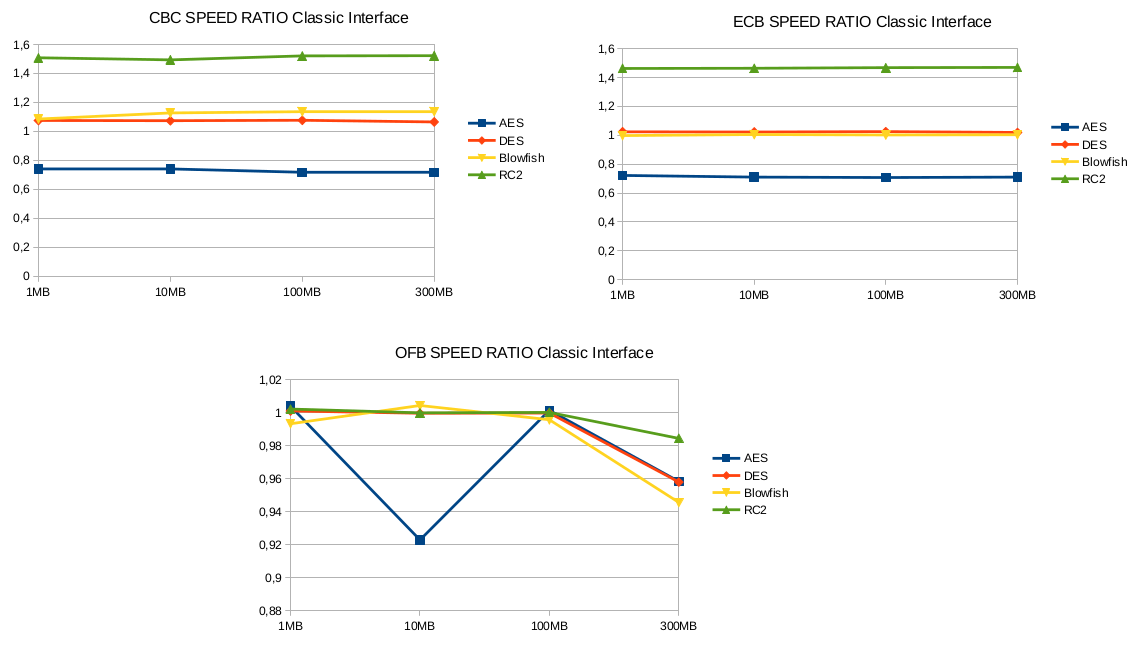
\includegraphics[width=1\textwidth]{pic2-hw1-1635747}
  \label{fig:Standard functions result}
\end{figure}

\subsection{EVP results}
Let's now analyze the results obtained with EVP.
The first graph immediately shows us a substantial difference with the previous results, the speed ratio of AES with CBC is close to 2,5. 
This is a much more accurate and real result than the one seen previously.

What happens when changing from CBC to ECB is the same result, ie AES with the ECB mode takes the same time both to decrypt and to encrypt.
Finally, we can see from the last graph that with OFB the speed ratio of the 4 ciphers does not change to before, and this makes us feel a little quieter. In the next section, we will explain the reason for these improvements in AES performance using the EVP interface and finally, in conclusion, we will try to answer the initial question.

\subsubsection{Why EVP is the right way}
As we said at the beginning, EVP is a high-level interface. In fact from the results seen, the performances improve.
But this happens above all for AES, why? Because EVP takes advantage of the AES-NI native instructions. To understand how AES-NI works, 
you need to think that to implement a crypto algorithm, we usually just express a combination of such basic operations additions, multiplications, XORs, and so on, and the microprocessor activates its adders, multipliers, and XOR circuits in the prescribed order. AES native instructions take this to a whole new level by providing developers with dedicated assembly instructions that compute AES. Instead of coding an AES round as a sequence of assembly instructions, when using AES-NI, you just call the instruction AESENC and the chip will compute the round for you. Native instructions allow you to just tell the processor to run an AES round instead of requiring you to program rounds as a combination of basic operations.
Running the simulation program we can see also that the speed of AES is higher than that with the standard functions. 
About the speed ratio, EVP is optimized and implements the parallelization of operations.

\begin{figure}[!ht]
  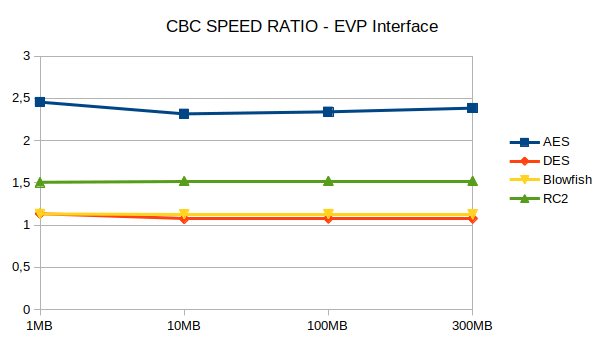
\includegraphics[width=1\textwidth]{pic3-hw1-1635747}
  \label{fig:CBC result- EVP interface}
\end{figure}
\begin{figure}
  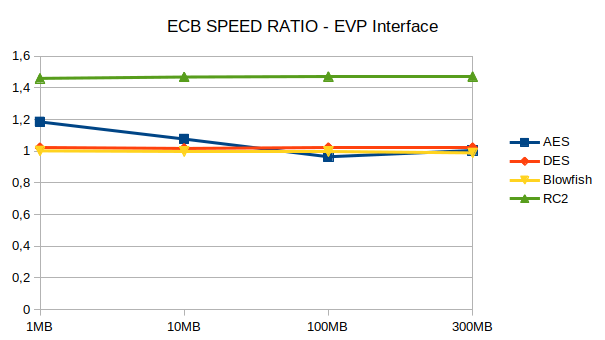
\includegraphics[width=1\textwidth]{pic4-hw1-1635747}
  \label{fig:ECB result- EVP interface}
\end{figure}
\begin{figure}
  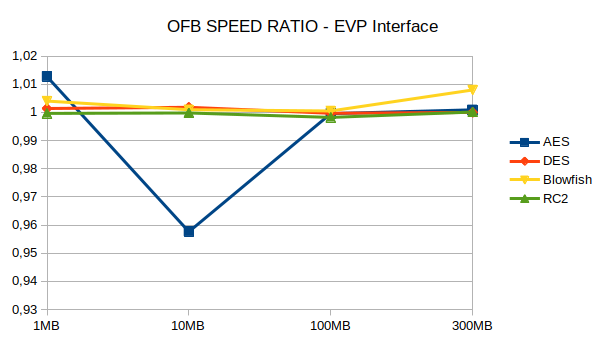
\includegraphics[width=1\textwidth]{pic5-hw1-1635747}
  \label{fig:OFB result- EVP interface}
\end{figure}

\newpage
\section{Conclusion}
Everything we have seen brings us to the following considerations: when you decide to encrypt or decrypt a file using OpenSSL it is always 
good to use the EVP interface because it increases performance and is optimized for AES.
Comparing the different ciphers we have seen that AES is by far the fastest, after which in the order we find Blowfish DES and RC2. 
The latter is the one that has the worst performance. By changing the operating modes the speed ratio changes, in particular, CBC makes 
the decryption faster, especially for AES, while OFB takes the same time both to decrypt and to encrypt whatever is the cipher used.
ECB is the fastest of the three.
Finally, changing the file size does not change the results significantly.

\begin{thebibliography}{99}

\bibitem{wiki}
{\em Block cipher mode of operation - Wikipedia}.
  \verb|https://en.wikipedia.org/wiki/Block_cipher_mode_of_operation|
  \newblock Accessed: 2019-11-4.

\bibitem{book}
Jean - Philippe Aumasson.
  {\em SERIOUS CRYPTOGRAPHY A Practical Introduction to Modern Encryption.}
  Copyright © 2018 by Jean-Philippe Aumasson.

\bibitem{link}
OpenSSL Documentation. 
{\em https://www.openssl.org/docs/manmaster/man3/}

\end{thebibliography}

\end{document}
